% 3. Data Corpus and Preprocessing Methodology
\section{The Need for Unification}
\label{ch:data_methodology}

This section presents an overview of the need for a unified framework for trajectory prediction in autonomous driving, addressing the challenges of dataset heterogeneity and the complexities of motion forecasting tasks. The discussion highlights the importance of standardizing data formats, feature characteristics, and preprocessing pipelines to enable effective model training and evaluation across diverse datasets.

\subsection{Unification of Motion Forecasting Datasets}
\label{sec:data_datasets}

The \texttt{UniTraj} framework addresses the fundamental challenge of standardizing multiple motion-forecasting datasets that exhibit substantial heterogeneities in both \emph{data formats} and \emph{feature characteristics}.
The former encompasses differences in data structure and organization, while the latter stems from variations in
spatio-temporal resolution, coverage range, and semantic annotation schemes.

To overcome format discrepancies, \texttt{UniTraj} leverages \texttt{ScenarioNet}~\cite{scenarionetLi2023} for conversion into a common
format, thereby eliminating the need for multiple preprocessing implementations. However, feature characteristics require additional harmonization. Temporal coverage varies substantially
across datasets, with historical trajectories ranging from 1 second in \texttt{WOMD}\cite{wmodSun2020} to 5 seconds in \texttt{Argoverse 2}\cite{av2Wilson2023},
and future prediction horizons extending from 6 to 8 seconds. Map resolutions and semantic annotations differ
significantly, with all datasets providing \emph{scene-centric} HD maps at varying resolutions.
Agent features also exhibit substantial variations: \texttt{nuScenes} provides only velocity and heading, while
\texttt{WOMD} includes comprehensive 3D bounding box annotations. Notably, \texttt{Argoverse 2} provides bounding
box and rich semantic annotations, but these are lost during \texttt{ScenarioNet} format conversion.
The conversion and normalization process is outlined in~\autoref{ssec:data_pipeline}.

\subsection{Unified ML Infrastructure}
Beyond dataset unification, trajectory prediction research requires a comprehensive machine learning infrastructure that handles the complexities of modern deep learning workflows. The UniTraj framework addresses this need by providing essential components that allow researchers to focus on model innovation rather than infrastructure implementation.

These components encompass the complete research pipeline: training and evaluation frameworks, data handling and preprocessing modules, logging and visualization tools, shared metrics and loss functions, and experiment management systems that facilitate reproducibility and systematic experimentation. Such a framework should be designed with transparency and modularity as core principles, enabling seamless extension and integration of new datasets, models, evaluation metrics, and additional functionalities such as callbacks or custom training procedures.



\subsection{Limitations of UniTraj}
\label{sec:data_challenges}

While we hoped to find a fully functional and well-structured implementation of the UniTraj framework, we encountered significant challenges that necessitated extensive refactoring and improvements to achieve a production-ready codebase.

The original UniTraj implementation suffered from critical software quality deficiencies that significantly hindered its usability and maintainability, as we had the goal to \emph{fully} understand the frameworks and its components that would be required to implement and train a model. Essentially the functionalities of the framework were mostly implemented but lacked transparency.

These issues included a lack of modular design patterns, insufficient type safety, and poor separation of concerns, which made the codebase difficult to navigate and extend. The absence of comprehensive documentation and standardized coding practices further exacerbated these problems, leading to confusion among developers and users alike.

When creating unified dataset, given multiple source datasets, they did not respect the original train, val, and test splits which is a common practice in machine learning

None of the most important symbols were annotated properly with type hints or explanatory comments or doc-strings. Especially the dataprocessing pipeline and the data handling were a single monolithic script with no clear separation of concerns, making it difficult to understand the data flow and transformations applied at each stage. The code lacked modular design patterns, leading to tight coupling between components and making it challenging to extend or modify the framework without introducing bugs which were annoying to deal with.
No proper separation of responsibilities, no modular design patterns.

None of the most important symbols and conventions used throughout this work, following UniTraj framework standards~\cite{unitrajFeng2024} and the \textsc{DatasetItem} type definitions.

While they were using \texttt{PyTorch Lightning}~\cite{falcon2019pytorch}, they were not following the recommended practices for employing it, such as using the \texttt{LightningDataModule} for data handling on the highest level, or a proper integration of logging functionalities such as Weights \& Biases with the framework.

Their path handling was poorly implemented, such that there was no clear control over the sources and destinations of various important data like the resulting datasets, model checkpoints and logs.

The training infrastructure lacked (and in some parts still lacks) essential deep learning capabilities: automatic mixed precision training, gradient accumulation, learning rate scheduling, and distributed computing support, various callbacks (such as learning rate monitors, early stopping, model checkpointing) all of which are easily configurable if using \texttt{PyTorch Lightning} in the way it's \emph{intended} to be used.

Another major issue was the lack of any typing information in the used \texttt{Hydra} configuration, which was essentially used as a dictionary without any type hints or structure, making it difficult to understand the effects of parameters or what kinds of values were expected. We decided to employ our own \emph{Config-as-Factory} pattern, where every functional component of the framework has it's own strongly typed configuration class that also serves as a factory for instantiating the corresponding component. This approach ensures type safety, improves code readability, and allows for various static analysis tools to catch potential issues early in the development process, as well as easy sanity checks when instantiating components like checking if all required parameters are in allowed ranges, if a path is valid, etc.



Mitigation strategies follow modern ML engineering best practices, with PyTorch Lightning migration as the primary solution. This architectural change provides structured training loops, automatic optimization, distributed computing support, and seamless experiment tracking integration~\cite{falcon2019pytorch}. Additional improvements include codebase refactoring into modular components, comprehensive unit and integration testing implementation, continuous integration adoption, and enhanced logging capabilities through Lightning's callback system for better visibility into training dynamics across datasets~\cite{unitrajFeng2024, scenarionetLi2023}.


\subsubsection{Revision of the UniTraj Framework}
This section details the major modifications we applied to the original UniTraj framework to achieve a more modular, type-safe, and production-ready codebase.

\paragraph{Data handling and preprocessing refinements.}
\begin{itemize}[leftmargin=*]
  \item \textbf{Strongly typed interfaces:} Introduced \href{https://github.com/JanDuchscherer104/UniTraj/blob/main/unitraj/datasets/types.py}{\texttt{types.py}} to declare all input and output tensors via \texttt{TypedDict} and dataclasses, replacing untyped \texttt{dict} passes and surfacing shape mismatches at static analysis time. Defines \texttt{RawScenarioDict}, \texttt{ProcessedDataDict} and other interfaces.
  \item \textbf{Decoupled parsing pipeline:} Split the monolithic script into three stages—\href{https://github.com/JanDuchscherer104/UniTraj/blob/main/unitraj/datasets/base_dataparser.py}{\texttt{base\_dataparser.py}} (handles raw file ingestion and basic conversions), \href{https://github.com/JanDuchscherer104/UniTraj/blob/main/unitraj/datasets/dataparser.py}{\texttt{dataparser.py}} (implements the nine-phase QC preprocessing pipeline), and \href{https://github.com/JanDuchscherer104/UniTraj/blob/main/unitraj/datasets/base_dataset.py}{\texttt{base\_dataset.py}} (wraps processed data into a PyTorch \texttt{Dataset} class), enabling modular parser swaps without code changes.
  \item \textbf{PyTorch Lightning integration:} Built a \href{https://github.com/JanDuchscherer104/UniTraj/blob/main/unitraj/lightning/lit_datamodule.py}{\texttt{lit\_datamodule.py}} (defines \texttt{LightningDataModule}) and \href{https://github.com/JanDuchscherer104/UniTraj/blob/main/unitraj/lightning/lit_trainer_factory.py}{\texttt{lit\_trainer\_factory.py}} (instantiates \texttt{pl.Trainer} from config) to configure \texttt{pl.Trainer} via YAML, unlocking multi-GPU, mixed-precision, and gradient accumulation.
  \item \textbf{Full Weights \& Biases (WandB) support:} Added comprehensive experiment tracking with real-time metric logging, hyperparameter sweeps, and model artifact management, enabling CSV dumps and real-time dashboards.
\end{itemize}

\paragraph{Architecture Overview}
The revised UniTraj framework follows a hierarchical configuration-driven architecture that enables modular component instantiation and type-safe data flow. Figure~\ref{fig:unitraj_data_architecture} illustrates the core data handling components and their relationships within the framework.

\begin{figure}[htbp]
    \centering
    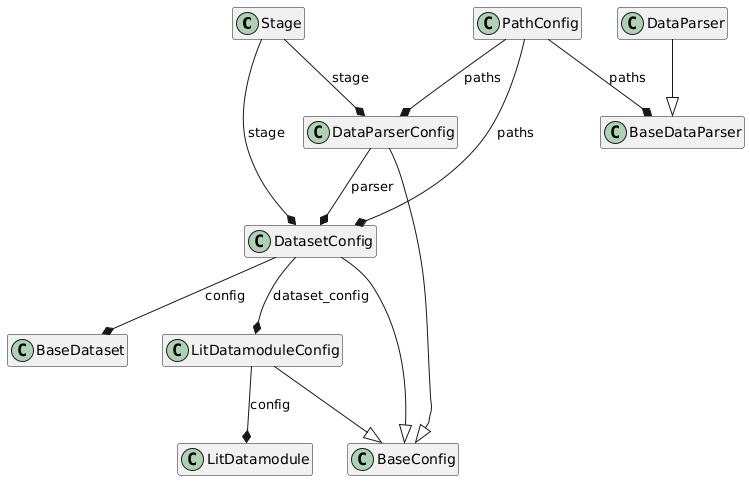
\includegraphics[width=0.9\textwidth]{figures/classes_DataHandling.png}
    \caption{UniTraj data handling architecture showing the relationships between configuration classes, data parsers, datasets, and Lightning modules. The diagram illustrates the Config-as-Factory pattern implementation and the modular data processing pipeline.}
    \label{fig:unitraj_data_architecture}
\end{figure}

The architecture comprises four primary layers:

\begin{itemize}[leftmargin=*]
    \item \textbf{Configuration Layer:} The \texttt{BaseConfig} class serves as the foundation for all configuration objects, implementing the Config-as-Factory pattern through the \texttt{setup\_target()} method. The \texttt{PathConfig} centralizes all filesystem paths and is automatically propagated to child configurations during instantiation. The \texttt{Stage} enum defines dataset splits (train/validation/test) and ensures consistent stage handling across the pipeline.
    \item \textbf{Data Processing Layer:} The \texttt{BaseDataParser} provides the interface for raw data ingestion, while \texttt{DataParser} implements the nine-phase preprocessing pipeline that transforms ScenarioNet format into normalized feature representations. The \texttt{DataParserConfig} controls preprocessing behavior including multiprocessing settings, cache management, and debug mode configuration.
    \item \textbf{Dataset Layer:} The \texttt{BaseDataset} wraps processed data into PyTorch-compatible format, implementing efficient data loading with optional H5PY file handles for large-scale datasets. The \texttt{DatasetConfig} manages dataset instantiation parameters and integrates the parser configuration for end-to-end data pipeline control.
    \item \textbf{Lightning Integration Layer:} The \texttt{LitDatamodule} provides PyTorch Lightning-compatible data loading with automatic train/validation/test split handling, configurable batch sizes, and multiprocessing support. The \texttt{LitDatamoduleConfig} enables declarative dataloader configuration from YAML files while maintaining type safety through Pydantic validation.
\end{itemize}

The composition relationships shown in the diagram reflect the framework's dependency injection approach: configurations contain references to their dependencies rather than hard-coded instantiations, enabling flexible component swapping and comprehensive testing. For instance, the \texttt{DatasetConfig} contains both a \texttt{DataParserConfig} and stage information, allowing different parsing strategies per dataset split without code duplication.

\paragraph{Configuration and path management.}
\begin{itemize}[leftmargin=*]
  \item \textbf{Config-as-Factory pattern:} Implemented \href{https://github.com/JanDuchscherer104/UniTraj/blob/main/unitraj/utils/base_config.py}{\texttt{base\_config.py}} (defines \texttt{BaseConfig} and \texttt{setup\_target()}) methods, allowing declarative instantiation of datasets, trainers, and models from YAML/JSON without touching code.
  \item \textbf{Centralized PathConfig:} Consolidated all filesystem paths (data root, logs, checkpoints) in \href{https://github.com/JanDuchscherer104/UniTraj/blob/main/unitraj/configs/path_config.py}{\texttt{path\_config.py}} (centralizes filesystem paths) and ensured automatic directory creation, eliminating scattered \texttt{os.makedirs()} calls.
  \item \textbf{Experiment reproducibility:} Integrated hierarchical overrides and \href{https://github.com/JanDuchscherer104/UniTraj/blob/main/unitraj/utils/base_config.py}{\texttt{base\_config.py}} (provides \texttt{inspect()} for config trees) to print the full resolved config tree at startup, improving traceability of parameter sweeps.
\end{itemize}

\paragraph{General refactoring and model zoo expansion.}
\begin{itemize}[leftmargin=*]
  \item \textbf{Modular model registry:} Refactored the \texttt{models/} folder into sub-packages (e.g., \texttt{autobot}, \texttt{mtr}, \texttt{wayformer}), each with its own \href{https://github.com/JanDuchscherer104/UniTraj/blob/main/unitraj/models/base_model/base_model.py}{\texttt{base\_model.py}} (defines \texttt{BaseModel} and \texttt{BaseModelConfig}), standardizing the interface for adding new architectures.
  \item \textbf{Utility consolidation:} Moved logging, console output, and visualization routines into \href{https://github.com/JanDuchscherer104/UniTraj/blob/main/unitraj/utils/console.py}{\texttt{console.py}} (provides structured \texttt{Console} API) modules, replacing ad-hoc print statements with a structured \texttt{Console} API.
  \item \textbf{Typed function signatures:} Audited all \texttt{.py} files to add precise type annotations for inputs and outputs (e.g., \texttt{batch: list[DatasetItem] -> BatchDict}), enabling \texttt{mypy} enforcement and catching runtime errors early.
\end{itemize}

\newpage